% $Header: /cvsroot/latex-beamer/latex-beamer/solutions/conference-talks/conference-ornate-20min.en.tex,v 1.6 2004/10/07 20:53:08 tantau Exp $

\documentclass{beamer}

% This file is a solution template for:

% - Talk at a conference/colloquium.
% - Talk length is about 20min.
% - Style is ornate.



%%%%%% New commands %%%%%%%
\newcommand\X{\mathcal{X}}
\newcommand\Z{\mathcal{Z}}
\newcommand\M{\mathcal{M}}
\newcommand\Lv{\mathcal{L}}
\newcommand\E{\mathbb{E}}
\newcommand\la{\ln{\bf \alpha}}
\newcommand{\Xcal}{\mathcal{X}}
\newcommand{\Zbf}{{\bf Z}}
\newcommand{\Vbf}{{\bf V}}
\newcommand{\Xbf}{{\bf X}}
\newcommand{\Zcal}{\mathcal{Z}}
\newcommand{\wbf}{{\bf w}}
\newcommand{\alphabf}{\text{\mathversion{bold}{$\alpha$}}}
\newcommand{\pibf}{\mbox{\mathversion{bold}{$\pi$}}}
\newcommand{\Pibf}{\mbox{\mathversion{bold}{$\Pi$}}}
\newcommand{\thetabf}{\mbox{\mathversion{bold}{$\theta$}}}
\newcommand{\Thetabf}{\mbox{\mathversion{bold}{$\Theta$}}}
\newcommand{\taubf}{\mbox{\mathversion{bold}{$\tau$}}}
\newcommand{\pibar}{\bar{\pi}}
\newcommand{\Qcal}{\mathcal{Q}}
\newcommand{\RX}{\mathcal{R}_{\Xbf}}
\newcommand{\Lcal}{\mathcal{L}}

%%%% tableau display\'{e}e \`{a} chaque case %%%%
\newenvironment{disarray}%
 {\everymath{\displaystyle\everymath{}}\array}%
 {\endarray}
%%%%%%%%%%%%%%%%%%

% Copyright 2004 by Till Tantau <tantau@users.sourceforge.net>.
%
% In principle, this file can be redistributed and/or modified under
% the terms of the GNU Public License, version 2.
%
% However, this file is supposed to be a template to be modified
% for your own needs. For this reason, if you use this file as a
% template and not specifically distribute it as part of a another
% package/program, I grant the extra permission to freely copy and
% modify this file as you see fit and even to delete this copyright
% notice.


\mode<presentation> {
  \usetheme[secheader]{Madrid}
  % or ...

  \setbeamercovered{transparent}
  \usefonttheme[onlymath]{serif} % pour les polices math\'{e}matiques avec serif
  \usecolortheme{crane}
  %\usefonttheme{serif}
  % or whatever (possibly just delete it)
}


\usepackage[english]{babel} %pour la langue fran\c{c}aise
\usepackage[latin1]{inputenc} % pour g\'{e}rer les polices latines
\usepackage[T1]{fontenc} % pour g\'{e}rer les accents
\usepackage{color,graphicx} % pour ins\'{e}rer des figures, mettre des accents
\usepackage{amssymb} % pour les symboles math\'{e}matiques
\usepackage{amsmath} % idem
\usepackage{amsfonts,txfonts} % idem
%\usepackage{pxfonts} % idem
\usepackage{bbm} %idem
\usepackage{hyperref} %pour cr\'{e}er automatiquement des liens hypertextes dans les r\'{e}f\'{e}rences
\usepackage{times}
% Or whatever. Note that the encoding and the font should match. If T1
% does not look nice, try deleting the line with the fontenc.


\title[Uncovering Structure in Valued Graphs] % (optional, use only with long paper titles)
{Uncovering Latent Structure in Valued Graphs}

%\subtitle
%{Include Only If Paper Has a Subtitle}

\author[Mariadassou] % (optional, use only with lots of authors)
{\underline{M.~Mariadassou}, S.~Robin}
% - Give the names in the same order as the appear in the paper.
% - Use the \inst{?} command only if the authors have different
%   affiliation.

\institute[AgroParisTech] % (optional, but mostly needed)
{
%  \inst{1}%
  UMR AgroParisTech/INRA MIA 518, Paris
%  \and
%  \inst{2}%
%  Projet HELIX, INRIA Rh\^{o}ne-Alpes
%  \and
%  \inst{3}%
%  UMR CNRS-8071/INRA-1152, Statistique et G\'{e}nome, \'Evry
}
% - Use the \inst command only if there are several affiliations.
% - Keep it simple, no one is interested in your street address.

\date[ECCS07] % (optional, should be abbreviation of conference name)
{ECCS07, October 2007}

% - Either use conference name or its abbreviation.
% - Not really informative to the audience, more for people (including
%   yourself) who are reading the slides online

\subject{Uncovering Structure in Biological Networks}
% This is only inserted into the PDF information catalog. Can be left
% out.

% If you have a file called "university-logo-filename.xxx", where xxx
% is a graphic format that can be processed by latex or pdflatex,
% resp., then you can add a logo as follows:

% \pgfdeclareimage[height=0.5cm]{university-logo}{university-logo-filename}
% \logo{\pgfuseimage{university-logo}}

% Delete this, if you do not want the table of contents to pop up at
% the beginning of each subsection:
%\AtBeginSection[] {
%  \begin{frame}<beamer>
%    \frametitle{Outline}
%    \tableofcontents[currentsection]
%  \end{frame}
%}

% If you wish to uncover everything in a step-wise fashion, uncomment
% the following command:

%\beamerdefaultoverlayspecification{<+->}

\begin{document}

\begin{frame}
  \titlepage
\end{frame}

\begin{frame}
  \frametitle{Outline}
  \tableofcontents
  % You might wish to add the option [pausesections]
\end{frame}


% Structuring a talk is a difficult task and the following structure
% may not be suitable. Here are some rules that apply for this
% solution:

% - Exactly two or three sections (other than the summary).
% - At *most* three subsections per section.
% - Talk about 30s to 2min per frame. So there should be between about
%   15 and 30 frames, all told.

% - A conference audience is likely to know very little of what you
%   are going to talk about. So *simplify*!
% - In a 20min talk, getting the main ideas across is hard
%   enough. Leave out details, even if it means being less precise than
%   you think necessary.
% - If you omit details that are vital to the proof/implementation,
%   just say so once. Everybody will be happy with that.

%%%%%%%%%%%%%%%%%%%%%%%%%%%%%%%%%%%%%%%%%%%%%%%%%%%%%%%%%%%%%%%%%%%%%%%
%%%%%%%%%%%%%%%%%%%%%%%%%%%%%%%%%%%%%%%%%%%%%%%%%%%%%%%%%%%%%%%%%%%%%%%
%%%%%%%%%%%%%%%%%%%%%%%%%%%%%%%%%%%%%%%%%%%%%%%%%%%%%%%%%%%%%%%%%%%%%%%
\section{Motivations}

%%%%%%%%%%%%%%%%%%%%%%%%%%%%%%%%%%%%%%%%%%%%%%%%%%%%%%%%%%%%%%%%%%%%%%%%
\begin{frame}
\frametitle{Motivations for the study of networks}
\begin{minipage}{.55\linewidth}
Networks\dots
\begin{itemize}
\item Arise in many fields:
\begin{itemize}
\item[\bf{$\rightarrow$}] Biology, Chemistry
\item[\bf{$\rightarrow$}] Physics, Internet.
\end{itemize}
\item Represent an interaction pattern:
\begin{itemize}
\item[\bf{$\rightarrow$}] $\mathcal{O}(n^2)$ interactions
\item[\bf{$\rightarrow$}] between $n$ elements.
\end{itemize}
\item Have a topology which:
\begin{itemize}
\item[\bf{$\rightarrow$}] reflects the structure/function
relationship
%\item[\bf{$\rightarrow$}]
\end{itemize}
\end{itemize}
\end{minipage}%
\begin{minipage}{0.45\linewidth}
\begin{center}
\includegraphics[width=\linewidth,angle=90]{figs/caida2_lg(brown).png}

\begin{tiny} From Barab\'asi website \end{tiny}
\end{center}
\end{minipage}
\end{frame}

%%%%%%%%%%%%%%%%%%%%%%%%%%%%%%%%%%%%%%%%%%%%%%%%%%%%%%%%%%%%%%%%%%%%%%%%
%%%%%%%%%%%%%%%%%%%%%%%%%%%%%%%%%%%%%%%%%%%%%%%%%%%%%%%%%%%%%%%%%%%%%%%%
%%%%%%%%%%%%%%%%%%%%%%%%%%%%%%%%%%%%%%%%%%%%%%%%%%%%%%%%%%%%%%%%%%%%%%%%
\section{An Explicit Random Graph Model}

%%%%%%%%%%%%%%%%%%%%%%%%%%%%%%%%%%%%%%%%%%%%%%%%%%%%%%%%%%%%%%%%%%%%%%%%
%%%%%%%%%%%%%%%%%%%%%%%%%%%%%%%%%%%%%%%%%%%%%%%%%%%%%%%%%%%%%%%%%%%%%%%%
\subsection{Some Notations}

%%%%%%%%%%%%%%%%%%%%%%%%%%%%%%%%%%%%%%%%%%%%%%%%%%%%%%%%%%%%%%%%%%%%%%%%
\begin{frame}
  \frametitle{Some Notations}
  %\framesubtitle{Subtitles are optional.}
  % - A title should summarize the slide in an understandable fashion
  %   for anyone how does not follow everything on the slide itself.
  \begin{itemize}
  \item
    \textbf{Notations:}
    \begin{itemize}
    \item[\bf{$\rightarrow$}] $V$ a set of vertices in $\{1,\dots,n\}$;\medskip
    \item[\bf{$\rightarrow$}] $E$ a set of edges in $\{1,\dots,n\}^2$;\medskip
    \item[\bf{$\rightarrow$}] $\Xbf=(X_{ij})$ the adjacency matrix, with
      $X_{ij}$ the value of the edge between $i$ and $j$.\medskip
    \end{itemize}
    % \item
    %   \textbf{Possible extensions}
    %   \begin{itemize}
    %   \item[\bf{$\rightarrow$}] Directed graphs: $X_{ij} \neq X_{ji}$
    %   \item[\bf{$\rightarrow$}] Valued graphs: $X_{ij} \in \mathbb{N}, \mathbb{R}$
    %   \end{itemize} \bigskip
  \item
    \textbf{Random graph definition:}
    \begin{itemize}
    \item[\bf{$\rightarrow$}] To describe the network, we need the joint distribution
    of the $X_{ij}$.
    \end{itemize}
    \medskip
    \pause
  \item
    \textbf{Example:}
    \begin{itemize}
    \item[]
      \begin{tabular}{cp{3.5cm}p{2.5cm}}
        \includegraphics[scale=0.3]{figs/Slide2.pdf} &
        \vspace{-1.25cm} \mbox{$V=\{1,2,3\}$} \mbox{$E=\left\{
            \{1,2\},\{2,3\},\{3,1\} \right\}$} &
        \vspace{-1.5cm}
        $
        \left(
          \begin{array}{ccc}
            . & 4 & 1 \\
            . & . & 2 \\
            . & . & . \\
          \end{array}
        \right)
        $
      \end{tabular}
    \end{itemize}
  \end{itemize}

\end{frame}

%%%%%%%%%%%%%%%%%%%%%%%%%%%%%%%%%%%%%%%%%%%%%%%%%%%%%%%%%%%%%%%%%%%%%%%%
%%%%%%%%%%%%%%%%%%%%%%%%%%%%%%%%%%%%%%%%%%%%%%%%%%%%%%%%%%%%%%%%%%%%%%%%
\subsection{Explicit Random Graph Model}

%%%%%%%%%%%%%%%%%%%%%%%%%%%%%%%%%%%%%%%%%%%%%%%%%%%%%%%%%%%%%%%%%%%%%%%%
% \begin{frame}
%   \frametitle{ER (Erd\"{o}s-R\'{e}nyi) Graph Model}
%   \begin{itemize}
%   \item
%     \textbf{The Model}
%     \begin{itemize}
%     \item[\bf{$\rightarrow$}] The oldest and best-known graph model,
%     \item[\bf{$\rightarrow$}] The $(X_{ij})$ are independent, with distribution
%       $\mathcal{B}(p)$.
%     \end{itemize}
%   \item
%     \textbf{Some Properties and Problems}
%     \begin{itemize}
%     \item[\bf{$\rightarrow$}] \alert{Degree} $K_i$ of a node $i$ has a Poisson distribution,
%       \[
%       K_i = \sum_{j \neq i} X_{ij} \sim \mathcal{P}(\lambda)
%       \]
%     \item[\bf{$\rightarrow$}] \alert{Clustering coefficient} $c$ is low: $c = p$
%       \[
%       c = \Pr\{X_{jk}=1|X_{ij}=X_{ik}=1\} = \Pr\{\nabla|\Vbf\}
%       \]
%     \item[\bf{$\rightarrow$}] Highly \alert{inaccurate} to describe real
%       networks.
%     \end{itemize}
%   \end{itemize}

% \end{frame}

%%%%%%%%%%%%%%%%%%%%%%%%%%%%%%%%%%%%%%%%%%%%%%%%%%%%%%%%%%%%%%%%%%%%%%%%
\begin{frame}
  \frametitle{Explicit Random Graph Model (vertices)}
  \begin{itemize}
  \item \textbf{Vertices heterogeneity}
    \begin{itemize}
    \item[\bf{$\rightarrow$}] Hypothesis: the vertices are distributed among $Q$ classes with
      different connectivity; \medskip
      \pause
    \item[\bf{$\rightarrow$}] $\Zbf=(\Zbf_i)_i$; \medskip
      $Z_{iq}=\mathbbm{1}\{i \in q\}$ are indep. hidden variables; \medskip
    \item[\bf{$\rightarrow$}] $\alphabf=\{\alpha_q\}$, the $prior$
      proportions of groups; \medskip
    \item[\bf{$\rightarrow$}] $(\Zbf_i)\sim \mathcal{M}(1,\alphabf)$.
    \end{itemize} \bigskip

    \pause
  \item
    \textbf{Example:}
    \begin{itemize}
    \item[\bf{$\rightarrow$}] Example for $8$ nodes and $3$ classes with
      $\alphabf=(0.25,0.25,0.5)$
      \begin{overprint}
        \onslide<1-2>
        \onslide<3->
        \includegraphics[scale=0.4]{figs/Slide3.pdf}
      \end{overprint}
    \end{itemize}
  \end{itemize}

\end{frame}

%%%%%%%%%%%%%%%%%%%%%%%%%%%%%%%%%%%%%%%%%%%%%%%%%%%%%%%%%%%%%%%%%%%%%%%%
\begin{frame}
  \frametitle{Explicit Random Graph Model (edges)}
  \begin{itemize}
  \item \textbf{$\Xbf$ distribution}
    \begin{itemize}
    \item[\bf{$\rightarrow$}] conditional distribution : $X_{ij}| \{i
      \in q, j \in \ell\} \sim f(.,\theta_{q\ell})$;\medskip
    \item[\bf{$\rightarrow$}] $\thetabf=(\theta_{q\ell})$ is the
      connectivity paramater matrix;\medskip
%    \item[\bf{$\rightarrow$}] ERMG : "Erd\"os-R\'{e}nyi Mixture for Graphs".
    \end{itemize}
    \medskip

    \pause
  \item \textbf{Example:}
    \begin{itemize}
    \item[\bf{$\rightarrow$}] Example for $3$ classes with
      Poisson-valued edges;
      % \item[\bf{$\rightarrow$}] Edge with value $0$ are not represented;
    \item[]
      \begin{overprint}
        \onslide<1>
        \onslide<2>
        \begin{center}
          \includegraphics[scale=0.4]{figs/Slide4a.pdf}
        \end{center}
        \onslide<3>
        \begin{center}
          \includegraphics[scale=0.4]{figs/Slide4b.pdf}
        \end{center}
        \onslide<4>
        \begin{center}
          \includegraphics[scale=0.4]{figs/Slide4c.pdf}
        \end{center}
        \onslide<5>
        \begin{center}
          \includegraphics[scale=0.4]{figs/Slide4d.pdf}
        \end{center}
        \onslide<6>
        \begin{center}
          \includegraphics[scale=0.4]{figs/Slide4e.pdf}
        \end{center}
        \onslide<7->
        \begin{center}
          \includegraphics[scale=0.4]{figs/Slide4f.pdf}
        \end{center}
      \end{overprint}
    \end{itemize}
  \end{itemize}
  \medskip

\end{frame}


%%%%%%%%%%%%%%%%%%%%%%%%%%%%%%%%%%%%%%%%%%%%%%%%%%%%%%%%%%%%%%%%%%%%%%%%
\begin{frame}
  \frametitle{Random Edge Values}
  \begin{itemize}
  \item \textbf{Classical Distributions:}
  \item[\bf{$\rightarrow$}] $f(.,\theta_{q\ell})$ can be \alert{any}
    probability distribution;\medskip
    \pause
  \item[\bf{$\rightarrow$}] Bernoulli: presence/absence of an
    edge;\medskip
    \pause
  \item[\bf{$\rightarrow$}] Multinomial: nature of the connection
    (friend, lover, colleague); \medskip
    \pause
  \item[\bf{$\rightarrow$}] Poisson: in coauthorship networks, number
    of copublished papers; \medskip
    \pause
  \item[\bf{$\rightarrow$}] Gaussian: intensity of the connection
    (airport network); \medskip
    \pause
  \item[\bf{$\rightarrow$}] Bivariate Gaussian: directed networks where
    forward and backward edges are correlated; \medskip
    \pause
  \item[\bf{$\rightarrow$}] Etc.
  \end{itemize}

  \pause
  \begin{center}
    \framebox{Mixture Model to easily generate graphs}
  \end{center}
\end{frame}

%%%%%%%%%%%%%%%%%%%%%%%%%%%%%%%%%%%%%%%%%%%%%%%%%%%%%%%%%%%%%%%%%%%%%%%%
% \begin{frame}
%   \frametitle{ERMG couterpart to some topologies}
%
%   %\vspace{-0.5cm}
%   \begin{table}[h]
%     \begin{center}
%       \begin{tabular}{lcccc}
%         \hline
%         Description & Network & $Q$ & $\pibf$
%         & \begin{tabular}{p{1.5cm}} Clustering coef. \end{tabular}\\
%         \hline
%         \begin{tabular}{p{2cm}} Random \end{tabular}
%         & \begin{tabular}{c}
%           \includegraphics[height=1.7cm,width=2.3cm]{figs/FigNetworks-Erdos.pdf}
%         \end{tabular}
%         & 1
%         &  $p$ & $p$ \\
%         % \hline
%         % \begin{tabular}{p{2cm}} Product connectivity (arbitrary degree
%         %   distribution) \end{tabular}
%         % & \begin{tabular}{c}\epsfig{file = figs/FigNetworks-Indep.eps,
%         %     height=2cm, width=4cm, clip=, bbllx=120, bblly=260, bburx=530,
%         %     bbury=570}  \end{tabular}
%         % & 2
%         % & $\left( \begin{array}{cc} a^2 &ab\\ ab&b^2\\ \end{array}
%         % \right)$
%         % & $\displaystyle{\frac{(a^2+b^2)^2}{(a+b)^2}}$ \\
%         \hline
%         \begin{tabular}{p{2cm}} Stars \end{tabular}
%         &
%         \begin{tabular}{c}
%           
\includegraphics[height=1.7cm,width=2.3cm]{figs/FigNetworks-Star.pdf}
%         \end{tabular}
%         & 4
%         & $\left( \begin{array}{cccc} 0&1&0&0\\ 1&0&1&0\\0&1&0&1\\0&0&1&0\\
%           \end{array} \right)$
%         & 0 \\
%         \hline \begin{tabular}{p{2cm}} Clusters (affiliation networks)
%         \end{tabular}

%         & \begin{tabular}{c}
%           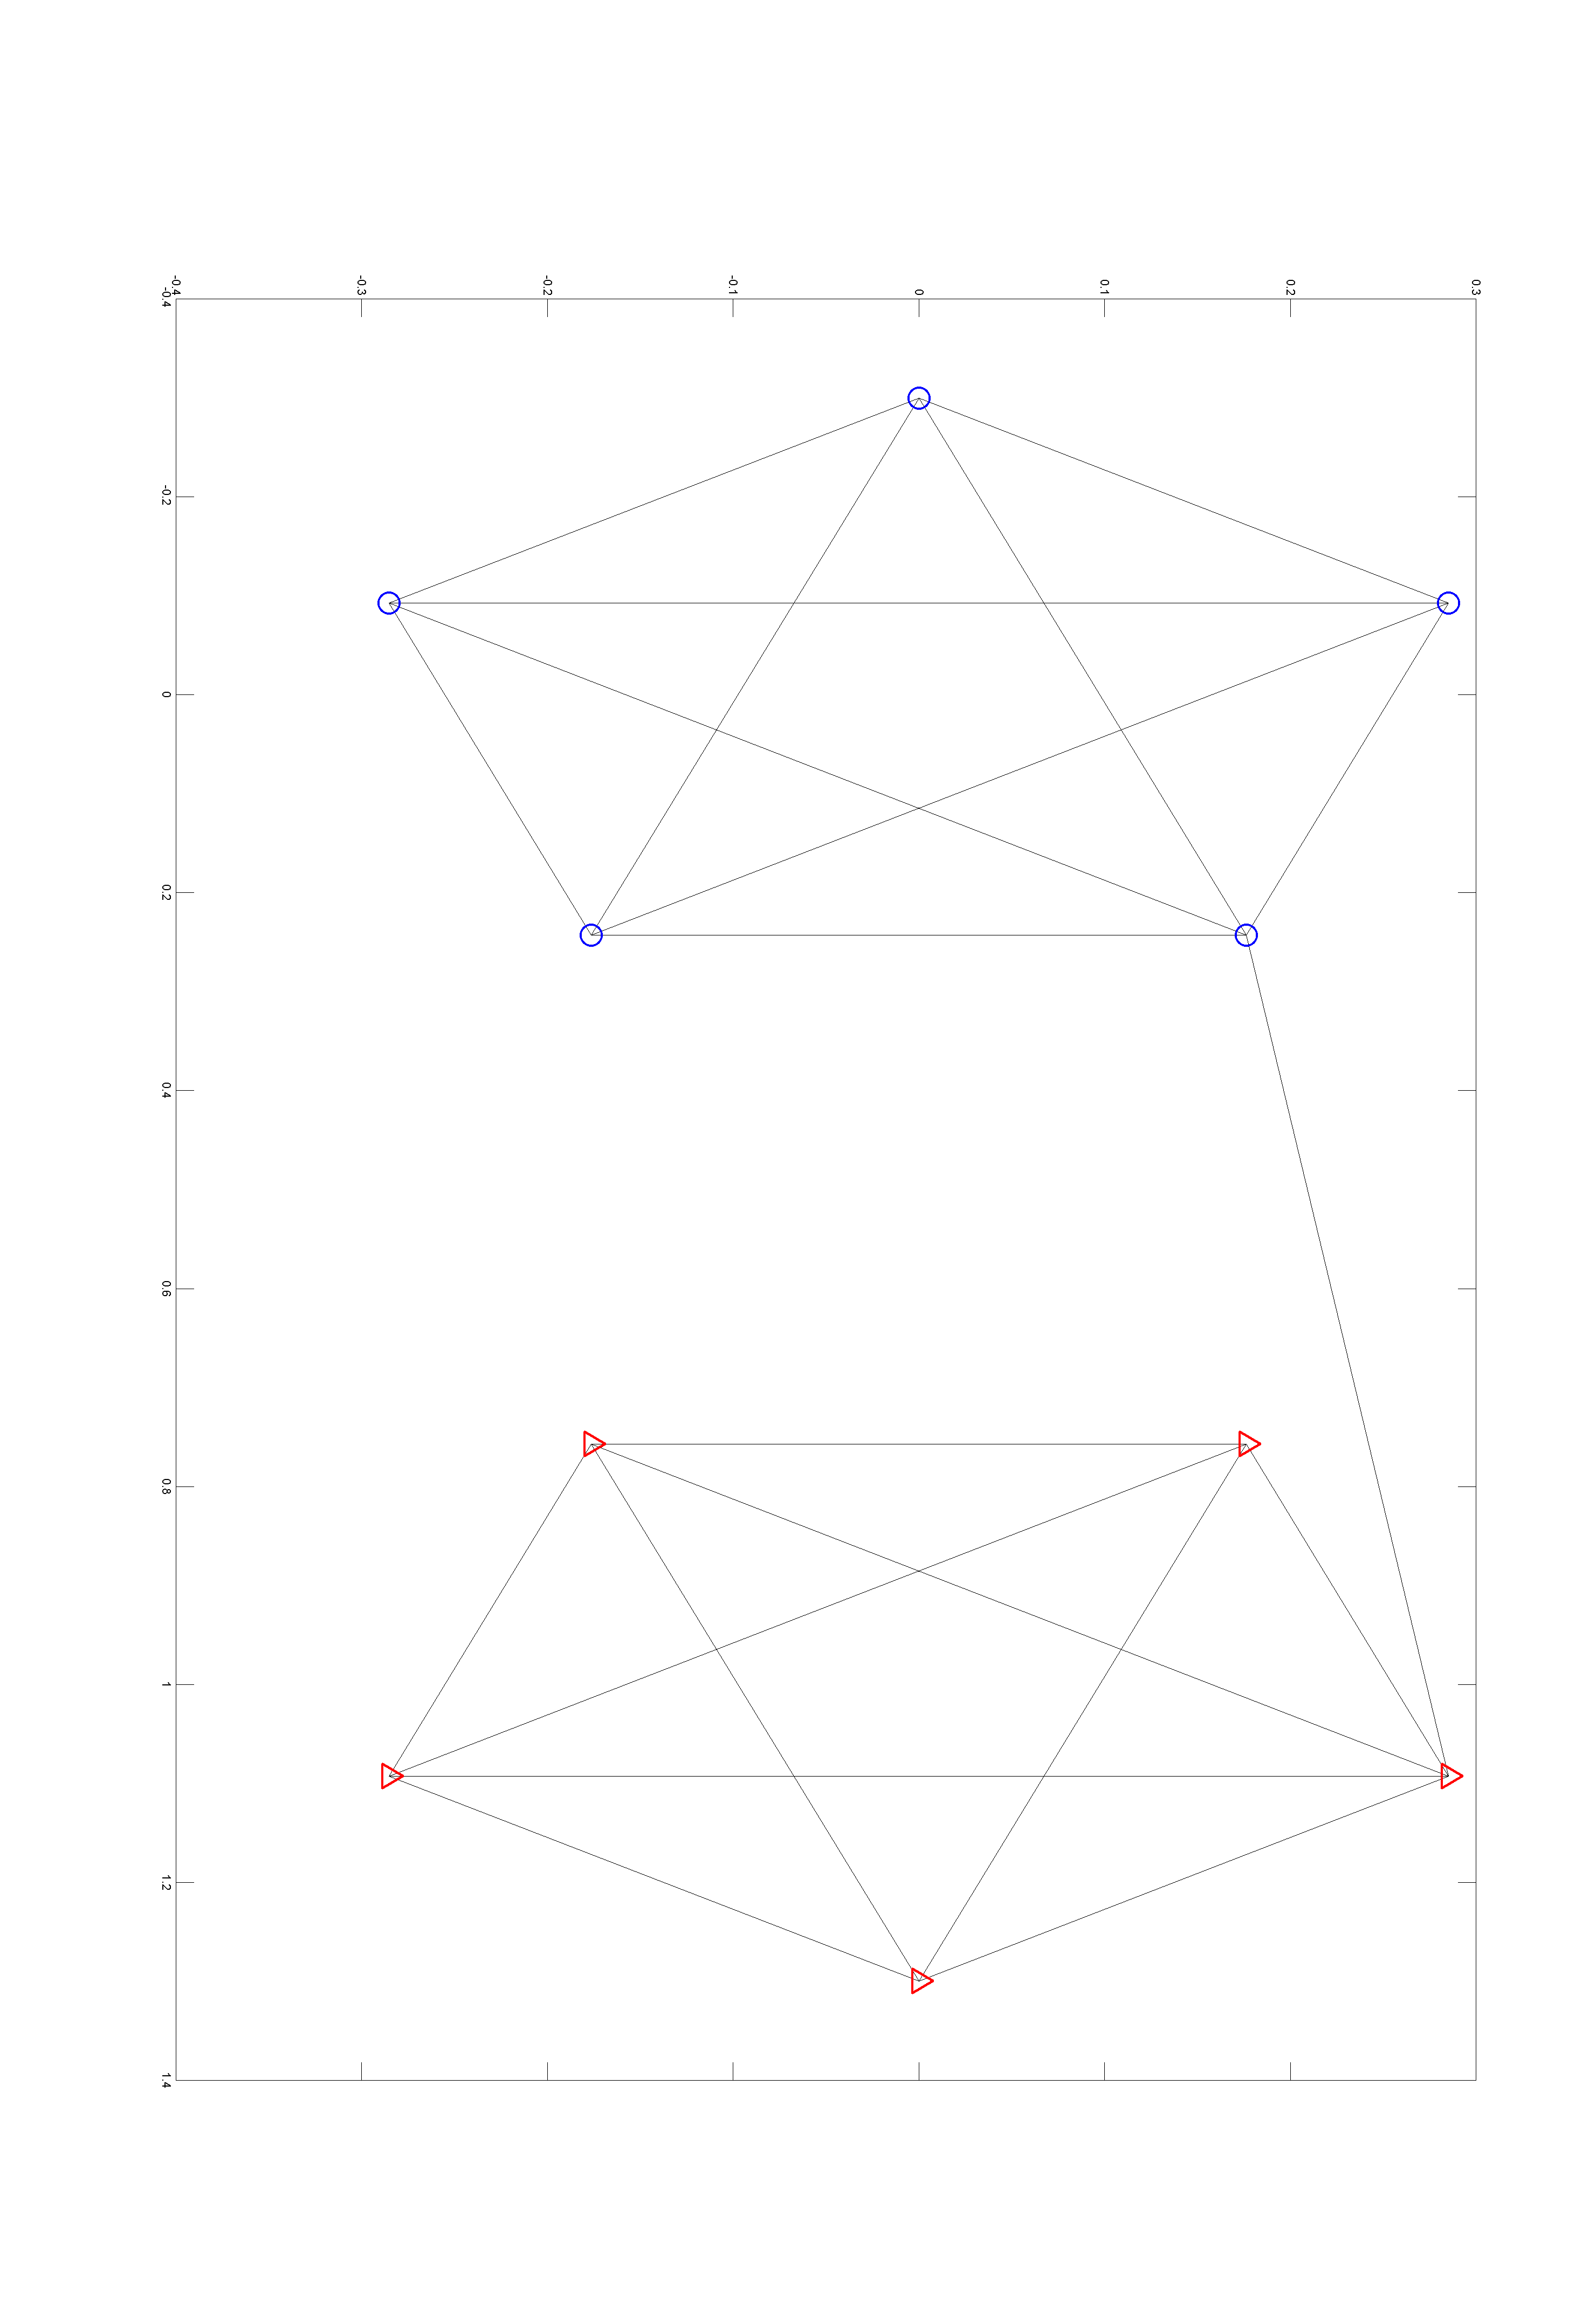
\includegraphics[height=1.7cm,width=2.3cm]{figs/FigNetworks-Clusters.pdf}
%         \end{tabular}
%         & 2
%         & $\left(\begin{array}{cc} 1&\varepsilon\\ \varepsilon&1\\
%           \end{array} \right)$ &
%         $\displaystyle{\frac{1+3\varepsilon^2}{(1+\varepsilon)^2}}$ \\
%         \hline
%       \end{tabular}
%     \end{center}
%   \end{table}

% \end{frame}


%%%%%%%%%%%%%%%%%%%%%%%%%%%%%%%%%%%%%%%%%%%%%%%%%%%%%%%%%%%%%%%%%%
%%%%%%%%%%%%%%%%%%%%%%%%%%%%%%%%%%%%%%%%%%%%%%%%%%%%%%%%%%%%%%%%%%
%%%%%%%%%%%%%%%%%%%%%%%%%%%%%%%%%%%%%%%%%%%%%%%%%%%%%%%%%%%%%%%%%%

\section{Parametric Estimation}

%%%%%%%%%%%%%%%%%%%%%%%%%%%%%%%%%%%%%%%%%%%%%%%%%%%%%%%%%%%%%%%%%%
%%%%%%%%%%%%%%%%%%%%%%%%%%%%%%%%%%%%%%%%%%%%%%%%%%%%%%%%%%%%%%%%%%
\subsection{Log-likelihoods and Variational Inference}

%%%%%%%%%%%%%%%%%%%%%%%%%%%%%%%%%%%%%%%%%%%%%%%%%%%%%%%%%%%%%%%%%%
\begin{frame}
  \frametitle{Log-Likelihood of the model}
  \textbf{First Idea:} Use maximum likelihood estimators
  \begin{itemize}
  \item \textbf{Complete data likelihood}
    \[
    \mathcal{L}(\Xbf,\Zbf) = \sum_i \sum_q Z_{iq}\ln{\alpha_q} +
    \sum_{i < j} \sum_{q,\ell} Z_{iq} Z_{j\ell}
    \ln{f_{\theta_{q\ell}}(X_{ij})}
    \]
    with $f_{\theta_{q\ell}}(X_{ij})$ likelihood of edge value
    $X_{ij}$ under $i \sim q$ and $j \sim \ell$.
    \pause
  \item \textbf{Observed data likelihood}
    \begin{center}
      $ \displaystyle \mathcal{L}(\Xbf) = \ln{\sum_{\Zbf}
        \exp{\mathcal{L}(\Xbf,\Zbf)}}
      $
    \end{center}
    \pause
  \item The observed data likelihood requires a sum over $Q^n$
    terms, and is thus \alert{untractable}; \medskip
  \item EM-like strategies require the knowledge of
    $\Pr(\Zbf|\Xbf)$, also untractable (no conditional independence) and thus also
    fail.
  \end{itemize}
\end{frame}

%%%%%%%%%%%%%%%%%%%%%%%%%%%%%%%%%%%%%%%%%%%%%%%%%%%%%%%%%%%%%%%%%%%%%%%%
\begin{frame}
  \frametitle{Variational Inference: Pseudo Likelihood}
  \textbf{Main Idea:} Replace \alert{complicated} $\Pr(\Zbf|\Xbf)$ by a \alert{simple} $\RX[\Zbf]$ such that
  $KL(\RX[\Zbf], \Pr(\Zbf|\Xbf))$ is minimal.\bigskip
  \pause
  \begin{itemize}
  \item Optimize in $\RX$ the function $\mathcal{J}(\RX)$ given by :
    \begin{eqnarray*}
      \mathcal{J}(\RX[\Zbf])  & = & \mathcal{L}(\Xbf)  - KL(\RX[\Zbf],
      \Pr(\Zbf|\Xbf)) \\
      & = & \mathcal{H}(\RX[\Zbf]) - \sum_{\Zbf} \RX[\Zbf]  \mathcal{L}(\Xbf,\Zbf)
    \end{eqnarray*}
  \end{itemize}
    \pause
  \begin{columns}
  \begin{column}{8cm}
  \begin{itemize}
  \item At best, $\RX = \Pr(\Zbf|\Xbf)$ and $\mathcal{J}(\RX[\Zbf])
    = \mathcal{L}(\Xbf)$;\bigskip
  \item For simple $\RX$, $\mathcal{J}(\RX[\Zbf])$ is tractable.
  \end{itemize}
  \end{column}
  \begin{column}{4cm}
    \begin{overprint}
    \onslide<1-2>
    \onslide<3->
    \includegraphics[width=3cm,heigth=3cm]{figs/Restriction.pdf}
    \end{overprint}
  \end{column}
  \end{columns}
\end{frame}

%%%%%%%%%%%%%%%%%%%%%%%%%%%%%%%%%%%%%%%%%%%%%%%%%%%%%%%%%%%%%%%%%%%%%%%%
%%%%%%%%%%%%%%%%%%%%%%%%%%%%%%%%%%%%%%%%%%%%%%%%%%%%%%%%%%%%%%%%%%%%%%%%
\subsection{Iterative Algorithm}

%%%%%%%%%%%%%%%%%%%%%%%%%%%%%%%%%%%%%%%%%%%%%%%%%%%%%%%%%%%%%%%%%%%%%%%%
\begin{frame}
  \frametitle{2 Step Algorithm}
  \begin{itemize}
  \item \alert{Step 1} \textbf{Optimize $\mathcal{J}(\RX[\Zbf])$ w.r.t.
    $\RX[\Zbf]$}:
    \begin{itemize}
    \item[\bf{$\rightarrow$}] Restriction to a "comfortable" class of
      functions;
    \item[\bf{$\rightarrow$}] $\RX[\Zbf]=\prod_i h(\Zbf_i;\taubf_{i,\Xbf})$,
      with $h(.;\taubf_{i,\Xbf})$ the multinomial distribution;
    \item[\bf{$\rightarrow$}] $\tau_{iq,\Xbf}$ is a variational parameter
      to be optimized using a fixed point algorithm:
      \begin{center}
        $
        \boxed{
          \tilde{\tau}_{iq,\Xbf} \propto \displaystyle \alpha_q
          \prod_{j \neq i} \prod_{\ell=1}^Q f_{\theta_{q\ell}}(X_{ij})^{\tilde{\tau}_{j\ell,\Xbf}}
        }
        $
      \end{center}
    \end{itemize}
    \bigskip
    \pause
  \item \alert{Step 2} \textbf{Optimize $\mathcal{J}(\RX[\Zbf])$ w.r.t.
      $(\alphabf,\thetabf)$}:
    \begin{itemize}
    \item[\bf{$\rightarrow$}] Constraint: $\sum_q \alpha_q =1$
      \begin{center}
        $
        \boxed{
          \begin{disarray}{rcl}
            \tilde{\alpha}_q & = & \sum_i \tilde{\tau}_{iq,\Xbf}/n \\
            \tilde{\theta}_{q\ell} & = & \arg\max_{\theta} \sum_{ij}
            \tilde{\tau}_{iq,\Xbf}\tilde{\tau}_{j\ell,\Xbf} \log{f_{\theta}(X_{ij})}
          \end{disarray}
        }
        $
      \end{center}
    \item[\bf{$\rightarrow$}] Closed expression of $\tilde{\theta}_{q\ell}$ for
      classical distributions.
    \end{itemize}
  \end{itemize}
\end{frame}

%%%%%%%%%%%%%%%%%%%%%%%%%%%%%%%%%%%%%%%%%%%%%%%%%%%%%%%%%%%%%%%%%%%%%%%%
%%%%%%%%%%%%%%%%%%%%%%%%%%%%%%%%%%%%%%%%%%%%%%%%%%%%%%%%%%%%%%%%%%%%%%%%
\subsection{Model Selection Criterion}

%%%%%%%%%%%%%%%%%%%%%%%%%%%%%%%%%%%%%%%%%%%%%%%%%%%%%%%%%%%%%%%%%%%%%%%%
\begin{frame}
  \frametitle{Model Selection Criterion}
  \begin{itemize}
  \item We derive a statistical BIC-like criterion to select the number of
    classes:\bigskip
  \item The likelihood can be split: $\Lcal(\Xbf, \Zbf |
    Q)=\Lcal(\Xbf | \Zbf,Q)  + \Lcal(\Zbf|Q)$.\bigskip
  \item These terms can be penalized separately:
    \begin{eqnarray*}
      \Lcal(\Xbf | \Zbf,Q) &\rightarrow &
      \text{pen}_{\Xbf|\Zbf}=\frac{Q(Q+1)}{2} \log \frac{n(n-1)}{2} \\
      \Lcal(\Zbf|Q)        &\rightarrow &  \text{pen}_{\Zbf} =
      (Q-1)\log(n)
    \end{eqnarray*}
  \end{itemize}

  \pause
  \begin{center}
    \framebox{$ICL(Q) = \underset{\thetabf}{\max} \Lcal(\Xbf ,
      \tilde{\Zbf} | \thetabf , m_Q) - \frac{1}{2}\left(\frac{Q(Q+1)}{2} \log
      \frac{n(n-1)}{2}- (Q-1) \log(n)\right)$}
  \end{center}
\end{frame}

%%%%%%%%%%%%%%%%%%%%%%%%%%%%%%%%%%%%%%%%%%%%%%%%%%%%%%%%%%%%%%%%%%
%%%%%%%%%%%%%%%%%%%%%%%%%%%%%%%%%%%%%%%%%%%%%%%%%%%%%%%%%%%%%%%%%%
%%%%%%%%%%%%%%%%%%%%%%%%%%%%%%%%%%%%%%%%%%%%%%%%%%%%%%%%%%%%%%%%%%

\section{Simulation Study}

%%%%%%%%%%%%%%%%%%%%%%%%%%%%%%%%%%%%%%%%%%%%%%%%%%%%%%%%%%%%%%%%%%
%%%%%%%%%%%%%%%%%%%%%%%%%%%%%%%%%%%%%%%%%%%%%%%%%%%%%%%%%%%%%%%%%%
\subsection{Quality of the estimates}

%%%%%%%%%%%%%%%%%%%%%%%%%%%%%%%%%%%%%%%%%%%%%%%%%%%%%%%%%%%%%%%%%%
\begin{frame}
  \frametitle{Simulation Setup}
  \begin{itemize}
  \item[\bf{$\rightarrow$}] Undirected graph with $Q=3$ classes;\medskip
    \pause
  \item[\bf{$\rightarrow$}] Poisson-valued edges;\medskip
    \pause
  \item[\bf{$\rightarrow$}] $n=100,\ 500$ vertices;\medskip
    \pause
  \item[\bf{$\rightarrow$}] $\alpha_q \propto a^q$ for $a=1,\ 0.5,\
    0.2$;
    \begin{itemize}
    \item $a=1$: balanced classes;
    \item $a=0.2$: unbalanced classes $(80.6\%,\ 16.1\%,\ 3.3\%)$
    \end{itemize}
    \pause
  \item[\bf{$\rightarrow$}] Connectivity matrix of the form
    $
    \left(
      \begin{array}{ccc}
        \lambda & \gamma \lambda & \gamma \lambda \\
        \gamma \lambda & \lambda & \gamma \lambda \\
        \gamma \lambda & \gamma \lambda & \lambda \\
      \end{array}
    \right)
    $
    for $\gamma = 0.1,\ 0.5,\ 0.9,\ 1.5$ and $\lambda = 2,\ 5$.
    \begin{itemize}
    \item $\gamma=1$: all classes equivalent (same connectivity pattern);
    \item $\gamma<>1$: classes are different;
    \item $\lambda$: mean value of an edge;
    \end{itemize}
    \item[\bf{$\rightarrow$}] $100$ repeats for each setup.
  \end{itemize}
\end{frame}

%%%%%%%%%%%%%%%%%%%%%%%%%%%%%%%%%%%%%%%%%%%%%%%%%%%%%%%%%%%%%%%%%%
\begin{frame}
  \frametitle{Results}
  \begin{itemize}
  \item $\text{Root Mean Square Error (RMSE)} = \sqrt{Bias^2 +
      Variance}$
  \end{itemize}
  \pause

\begin{overprint}
\onslide<1>
\onslide<2->
    \begin{center}
      \begin{tabular}{lr}
        RMSE for the $\alpha_q$ & RMSE for the
        $\lambda_{ql}$ \\
        $x$-axis: $\alpha_1, \alpha_2,\alpha_3$ & $x$-axis:
        $\lambda_{11}, \lambda_{22}, \lambda_{33}, \lambda_{12},
        \lambda_{13}, \lambda_{23}$\\
        \includegraphics[bb=50 100 600 700,scale=0.2]{figs/AlphaRMSE.pdf} &
        \includegraphics[bb=620 250 250 750,scale=0.2,angle=270]{figs/LambdaRMSE.pdf} \\
      \end{tabular}

    ($n$,$\lambda$,$\gamma$,$a$) from left (hard) to right (easy):
    $(100,2,0.9,0.2),\ (100,2,0.5,0.5),\ (500,5,0.1,1)$
  \end{center}
\end{overprint}

\end{frame}

%%%%%%%%%%%%%%%%%%%%%%%%%%%%%%%%%%%%%%%%%%%%%%%%%%%%%%%%%%%%%%%%%%
%%%%%%%%%%%%%%%%%%%%%%%%%%%%%%%%%%%%%%%%%%%%%%%%%%%%%%%%%%%%%%%%%%
 \subsection{Number of Classes}

%%%%%%%%%%%%%%%%%%%%%%%%%%%%%%%%%%%%%%%%%%%%%%%%%%%%%%%%%%%%%%%%%%
\begin{frame}
  \frametitle{Simulation Setup and Results}

\begin{columns}
   \begin{column}{0.6\linewidth}
    \begin{itemize}
    \item[\bf{$\rightarrow$}] Undirected graph with $Q^\star=3$ classes;\medskip
    \item[\bf{$\rightarrow$}] Poisson-valued edges;\medskip
    \item[\bf{$\rightarrow$}] $n=50,\ 100,\ 500,\ 1000$ vertices;\medskip
    \item[\bf{$\rightarrow$}] $\alpha_q = (57.1\%,28,6\%,14,3\%)$ (or
    $a=0.5$);\medskip
    \item[\bf{$\rightarrow$}] $\lambda = 2, \gamma = 0.5$; \medskip
    \item[\bf{$\rightarrow$}] Retrieve $Q$ that maximizes ICL;\medskip
    \item[\bf{$\rightarrow$}] $100$ repeats for each value of $n$;
    \end{itemize}
   \end{column}

   \begin{column}{0.4\linewidth}
  \uncover<2->{
      \begin{tabular}{|c|ccc|}
        \cline{2-4}
        \multicolumn{1}{c}{} & \multicolumn{3}{|c|}{$Q$} \\
        \hline
        $n$ & 2 & 3 & 4 \\
        \hline
        50 & 82 & \textbf{17} & 1 \\
        100 & 7 & \textbf{90} & 3 \\
        500 & 0 & \textbf{100} & 0 \\
        1000 & 0 & \textbf{100} & 0 \\
        \hline
      \end{tabular}
      Frequency (in \%) at which Q is selected for various
        $n$.
  }
  \end{column}
\end{columns}

\end{frame}

%%%%%%%%%%%%%%%%%%%%%%%%%%%%%%%%%%%%%%%%%%%%%%%%%%%%%%%%%%%%%%%%%%
%\begin{frame}
%  \frametitle{Number of Classes: Results}
%
%  \begin{figure}
%    \begin{tabular}{cccc}
%      \includegraphics[bb=49 91 529 757,scale=0.1]{figs/Fig-ICL_n_50.pdf} &
%      \includegraphics[bb=49 91 529 757,scale=0.1]{figs/Fig-ICL_n_100.pdf} &
%      \includegraphics[bb=38 94 529 757,scale=0.1]{figs/Fig-ICL_n_500.pdf} &
%      \includegraphics[bb=38 100 529 754,scale=0.1]{figs/Fig-ICL_n_1000.pdf}
%    \end{tabular}
%    \caption{Mean ICL and 90\% confidence interval as a function of
%      $Q=1..10$. From left to right: $n=50, n=100, n=500, n=1000$.}
%  \end{figure}
%
%\pause
%
%  \begin{table}[h]
%    \begin{center}
%      \begin{tabular}{|c|ccc|}
%        \cline{2-4}
%        \multicolumn{1}{c}{} & \multicolumn{3}{|c|}{$Q$} \\
%        \hline
%        $n$ & 2 & 3 & 4 \\
%        \hline
%        50 & 82 & \textbf{17} & 1 \\
%        100 & 7 & \textbf{90} & 3 \\
%        500 & 0 & \textbf{100} & 0 \\
%        1000 & 0 & \textbf{100} & 0 \\
%        \hline
%      \end{tabular}
%      \caption{Frequency (in \%) at which Q is selected for various
%        $n$.}
%    \end{center}
%  \end{table}
%\end{frame}

%%%%%%%%%%%%%%%%%%%%%%%%%%%%%%%%%%%%%%%%%%%%%%%%%%%%%%%%%%%%%%%%%%%%%%%%
%%%%%%%%%%%%%%%%%%%%%%%%%%%%%%%%%%%%%%%%%%%%%%%%%%%%%%%%%%%%%%%%%%%%%%%%
%%%%%%%%%%%%%%%%%%%%%%%%%%%%%%%%%%%%%%%%%%%%%%%%%%%%%%%%%%%%%%%%%%%%%%%%
\section*{Summary}

%%%%%%%%%%%%%%%%%%%%%%%%%%%%%%%%%%%%%%%%%%%%%%%%%%%%%%%%%%%%%%%%%%%%%%%%
\begin{frame}
  \frametitle<presentation>{Summary}

  % Keep the summary *very short*.
  \begin{block}{Flexibility of ERMG}
  \begin{itemize}
  \item A simple way to simulate networks;
  \item Many distributions to model different networks;
  \item Probabilistic model which captures features of real-networks (data
  not-shown).
  \end{itemize}
  \end{block}

  \begin{block}{Estimation and Model selection}
  \begin{itemize}
  \item Variational approaches to compute approximate MLE when
  dependencies are complex,
  \item A statistical criterion to choose the number of classes
  (ICL).
  \end{itemize}
  \end{block}

\end{frame}


\section*{Discussion}

%%%%%%%%%%%%%%%%%%%%%%%%%%%%%%%%%%%%%%%%%%%%%%%%%%%%%%%%%%%%%%%%%%%%%%%%
\begin{frame}
  \frametitle{\emph{E. Coli} reaction network \texttt{http://www.biocyc.org/}}
  \begin{minipage}{.5\linewidth}
    \begin{itemize}
    \item Dot-plot representation ($605$ nodes and $1,782$ vertices)
      \begin{itemize}
      \item[\bf{$\rightarrow$}] adjacency matrix (sorted)
      \end{itemize}
    \item Biological interpretation:
      \begin{itemize}
      \item[\bf{$\rightarrow$}] Groups 1 to 20 gather reactions
        involving all the \alert{same compound} either as a substrate or
        as a product,
      \item[\bf{$\rightarrow$}] A compound (chorismate, pyruvate,
        ATP,\emph{etc}) can be associated to each group.
      \end{itemize}
    \item The structure of the metabolic network is governed by the
      compounds.
    \end{itemize}
  \end{minipage}%
  \begin{minipage}{.5\linewidth}
    \begin{center}
      \includegraphics[width=5cm,height=5cm,angle=90]{figs/Ecoli-Complet-ERMG-Ward-Q21_class2.pdf}
    \end{center}
  \end{minipage}%

\end{frame}

%%%%%%%%%%%%%%%%%%%%%%%%%%%%%%%%%%%%%%%%%%%%%%%%%%%%%%%%%%%%%%%%%%%%%%%%
\begin{frame}
  \frametitle{\emph{E. Coli} reaction network \texttt{http://www.biocyc.org/}}
  \begin{minipage}{.5\linewidth}
    \begin{itemize}
    \item[\bf{$\rightarrow$}] Classes 1 and 16 constitute s single
      clique corresponding to a single compound (pyruvate),
    \item[\bf{$\rightarrow$}] They are split into two classes
      because they interact differently with classes 7 (CO2) and 10
      (AcetylCoA)
    \item[\bf{$\rightarrow$}] Connectivity matrix (sample):
      $
      \begin{array}{c|cccc}
        q, l & 1 & 7 & 10 & 16 \\
        \hline
        1  & \textcolor{red}{1.0} & & & \\
        7  & \textcolor{green}{.11} & .65 & &  \\
        10 & \textcolor{green}{.43} & & .67 & \\
        16 & \textcolor{red}{1.0} & \textcolor{yellow}{.01} &
        \textcolor{yellow}{\epsilon} & \textcolor{red}{1.0}
      \end{array}
      $
    \end{itemize}
  \end{minipage}%
  \begin{minipage}{.5\linewidth}
    \begin{center}
      \includegraphics[width=5cm,height=5cm,angle=90]{figs/Ecoli-Complet-ERMG-Ward-Q21_class3.pdf}
      \begin{tiny} Adjacency matrix (sample) \end{tiny}
    \end{center}
  \end{minipage}%

\end{frame}



%  % The following outlook is optional.
%  \vskip0pt plus.5fill
%  \begin{itemize}
%  \item
%    Outlook
%    \begin{itemize}
%    \item
%      Something you haven't solved.
%    \item
%      Something else you haven't solved.
%    \end{itemize}
%  \end{itemize}
%\end{frame}



% All of the following is optional and typically not needed.
%\appendix
%\section<presentation>*{\appendixname}
%\subsection<presentation>*{For Further Reading}
%
%\begin{frame}[allowframebreaks]
%  \frametitle<presentation>{For Further Reading}
%
%  \begin{thebibliography}{10}
%
%%  \beamertemplatebookbibitems
%%  % Start with overview books.
%
%  \beamertemplatearticlebibitems
%  % Followed by interesting articles. Keep the list short.
%  \bibitem{Jaakkola00tutorial}
%    T.~Jaakkola
%    \newblock {\em Tutorial on variational approximation methods}.
%    \newblock MIT Press, 2000.
%
%  \bibitem{Snijders2001}
%  Kryztof Nowicki and Tom A.~B.~Snijders
%  \newblock Estimation and Prediction for Stochastic Blockstructures
%  \newblock \emph{Journal of the American Statistical Association},
%  96(455):1077--1087,2001.
%
%  \bibitem{leisink01tighter}
%    M.~Leisink and H.~Kappen
%    \newblock A Tighter Bound for Graphical Models
%    \newblock {\em Neural Computation}, 13(9):2149--2171,
%    2001.
%  \end{thebibliography}
%\end{frame}

\end{document}
